\chapter{Methodology II and Experimental Design}
\label{chap:experimental_design}

This chapter defines the final experimental frame of the thesis and presents the second methodological line built on top of the earlier controller-centered baseline. The paper-facing experimental backbone remains the retained controller-line scope, but the chapter also introduces the dynamic-shadow-price integrated solver developed in the fresh-solver line. The purpose is therefore twofold: first, to state clearly which experiments define the stable thesis evidence structure; second, to explain how the newer integrated solver line is evaluated without collapsing it into a flat ranking against the retained controller line.

\section{Retained paper-facing experiment scope}

The stable paper-facing scope of the thesis is intentionally narrow. It is anchored in two baseline experiment settings, \texttt{EXP00} and \texttt{EXP01}, and in the \texttt{Scenario1} controller progression built on top of \texttt{EXP01}. This retained scope is the result of the methodological narrowing discussed in Chapter~\ref{chap:methodological_evolution}: it keeps the experimental story interpretable, reproducible, and safe to write about.

Within this scope, \texttt{EXP00} serves as the normal operating reference, while \texttt{EXP01} defines a pressure scenario in which service deterioration becomes visible. The retained method line is then written as a controller progression over \texttt{Scenario1}, following the sequence \texttt{v2} $\rightarrow$ \texttt{v4} $\rightarrow$ \texttt{v5} $\rightarrow$ \texttt{v6f} $\rightarrow$ \texttt{v6g}. According to the writing map and claim guardrails, this progression forms the main paper-facing method chain. In particular, \texttt{v6g} is the current canonical Herlev main candidate, \texttt{v6f} is the mechanism transition into execution-aware control, and variants such as \texttt{cap05}, \texttt{automode}, or \texttt{v6b3} are interpreted as supplementary or counterexample lines rather than as replacements for the canonical endpoint.

This framing is important because the later integrated-solver work does not invalidate the retained controller-centered evidence. Instead, it extends the thesis by sharpening how depot-aware realism is modeled and how difficult instances should be interpreted. The retained controller-line results therefore remain the reference line for the paper-facing experimental narrative, while the newer fresh-solver results are evaluated as a complementary integrated method line.

\section{Benchmark instances and regime structure}

The integrated-solver experiments focus on three benchmark instances that naturally expose different operational regimes: Herlev, East, and West. They differ substantially in both scale and pressure structure, making them useful not only for performance comparison but also for diagnostic interpretation.

Herlev is the medium-pressure instance. It is small enough to remain analytically transparent, yet rich enough to display meaningful interactions between rolling admission, routing feasibility, and depot-resource pressure. For this reason, Herlev is especially useful for controlled method progression and for comparing retained controller-centered variants.

East is a larger but relatively looser instance. Under the current integrated-solver setup, East already performs very strongly under earlier OR-style baselines, which makes it a good test of whether an intervention adds genuine value or merely introduces unnecessary conservatism. In other words, East functions as the low-pressure or already-near-feasible regime.

West is the most difficult instance and the most important one for the dynamic-shadow-price line. It combines larger scale with strong depot-side pressure, especially in warehouse picking. Earlier diagnostics show that West is dominated not by all-day capacity shortage, but by a sharply localized morning wave. West therefore functions as the high-pressure, wave-dominant regime in which the integrated solver is most clearly stress-tested.

This high/medium/low pressure interpretation should not be read as a rigid theoretical taxonomy. Rather, it is an empirical organizing principle that helps explain why some methods generalize smoothly while others become regime-dependent. In the thesis, this regime structure is central to understanding the value and limits of the dynamic-shadow-price mechanism.

\section{Methodology II: dynamic shadow-price integrated solver}

Methodology II takes the integrated controller-routing-repair architecture seriously as the main solver object. Instead of relying mainly on controller-side clipping and protection, it tries to internalize depot pressure more explicitly into the route-construction process itself. The key mechanism is a dynamic shadow-price signal defined over depot time buckets and resource types.

At a high level, the idea is to treat high-utilization resource buckets as expensive states. When diagnostics indicate that a specific 15-minute bucket is close to or beyond its practical capacity, inserting new workload into that bucket should incur a higher marginal cost. In this way, the solver no longer reacts to depot pressure only after a route set has been constructed. Instead, the route builder is guided away from particularly dangerous buckets while the controller can also reduce the admission of demand that would further worsen those same high-pressure intervals.

The mechanism is dynamic because the price signal is not fixed globally. It is generated from bucket-level utilization diagnostics and can vary across resource types such as gate, picking, and staging. In the present thesis line, picking pressure is the most important resource signal, especially on West, but the architecture is designed so that depot pressure can in principle be represented in a common pricing language rather than through hand-written, instance-specific rules.

The integrated solver therefore combines three effects. First, the controller can still protect urgent demand and clip especially risky flexible demand. Second, the routing layer uses insertion costs that now include depot-aware marginal penalties rather than relying only on transportation feasibility and travel cost. Third, the repair layer remains available to reduce residual overload after route construction. The dynamic-shadow-price method is thus not a separate module bolted onto routing; it is a cross-layer coordination mechanism inside the integrated controller-routing-repair architecture.

Figure~\ref{fig:integrated_architecture} shows this architecture in a condensed form. The main purpose of the figure is to make clear that the fresh-solver line is not just ``a better route builder,'' but a coordinated rolling system in which admission control, routing, and depot repair exchange information across the day.

\begin{figure}[tbp]
    \centering
    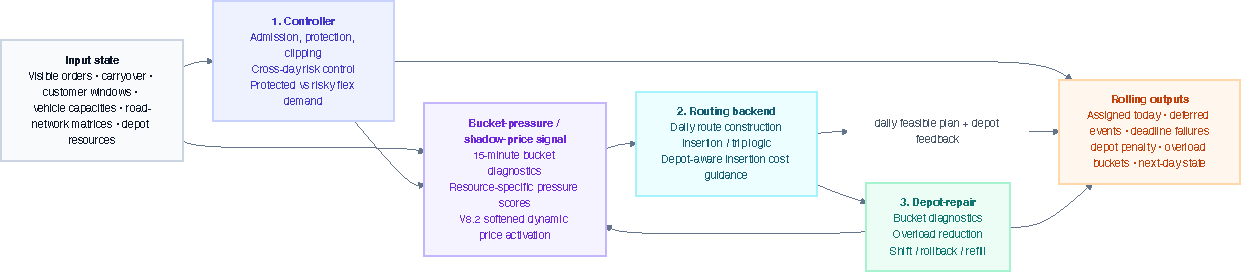
\includegraphics[width=0.96\textwidth]{Pictures/professor_preview/fig_integrated_architecture.pdf}
    \caption{Figure 6.1 shows the integrated planning architecture used in the fresh-solver line. In the V8.2 branch, bucket-level depot diagnostics are converted into a bucket-pressure / shadow-price signal that feeds depot-aware routing guidance, while the controller and depot-repair layers continue to shape exposure and reduce residual overload before the system rolls to the next day.}
    \label{fig:integrated_architecture}
\end{figure}

This architectural view also helps explain why the dynamic-shadow-price mechanism belongs in the methodology chapter rather than being treated as a late implementation detail. It is a structural feature of the integrated line, not merely a local routing tweak.

\section{From V8 to V8.1 to V8.2}

The V8 line is best understood as a scientific progression rather than as a sequence of arbitrary parameter changes. The first V8 version established the central proof of concept: bucket-level dynamic prices do change route structure and can reshape the depot workload curve. This is an important result in itself, because it shows that dynamic depot pricing is not merely decorative. However, the first version also showed that overly aggressive price activation can degrade service badly and shift the bottleneck rather than solving it. On West, V8 reduced the original morning spike only by pushing too much pressure into a later 08:00--09:00 wave while service rate collapsed sharply.

V8.1 was designed as a correction to that over-control. It reduced the harshness of controller clipping and softened the routing-side price signal. The result was a partial recovery: the original 06:00 spike was visibly reduced, total and morning picking overload dropped below the earlier OR-V7 level, and service recovered substantially. At the same time, V8.1 still exhibited an undesirable secondary peak, meaning that the wave-shaping logic was moving in the right direction but had not yet found the best balance.

V8.2 represents the current best point on this line. It further relaxes dynamic price intensity and controller hardening while preserving the bucket-aware smoothing mechanism. On West, this produces the best service--smoothing trade-off so far: service rises to approximately 99.41\%, while both total and morning picking overload fall below OR-V7. In curve terms, the original 06:00 wave is materially reduced without being simply displaced into a new late-morning overload cluster. For the thesis, this makes V8.2 the main representative of the dynamic-shadow-price line.

The V8 progression therefore supports a stronger methodological claim than ``parameter tuning improved performance.'' More precisely, it shows that bucket-level dynamic prices are powerful enough to reshape route structures, that uncontrolled activation can create harmful peak migration, and that useful smoothing requires a calibrated balance between depot protection and throughput preservation.

\section{Evaluation metrics and aligned KPI schema}

Because the thesis includes both a retained controller-centered line and a newer integrated solver line, evaluation requires two layers of metrics. The first layer is a paper-facing aligned schema that allows readable cross-system comparison at the top level. The second layer preserves system-native diagnostics that reveal process structure and should not be discarded merely for the sake of a common table.

The aligned top-level KPI schema consists of four fields:
\begin{itemize}
    \item total eligible orders (\texttt{eligible\_count}),
    \item delivered orders within window (\texttt{delivered\_within\_window\_count}),
    \item deadline failures (\texttt{deadline\_failure\_count}), and
    \item within-window service rate (\texttt{service\_rate\_within\_window}).
\end{itemize}
These fields capture the most important service outcome in a common language: out of all eligible unique orders in the horizon, how many were completed on time and how many failed by their deadline. This schema is shared across the retained and integrated lines and is the safest basis for thesis-level readable comparison.

At the same time, the integrated solver line tracks additional native process metrics:
\begin{itemize}
    \item total deferred events (\texttt{total\_deferred\_events}),
    \item final carryover orders (\texttt{final\_carryover\_orders}),
    \item depot penalty (\texttt{depot\_penalty}), and
    \item overload-bucket count (\texttt{overload\_bucket\_count}).
\end{itemize}
These are not secondary bookkeeping artifacts. They encode whether service is being protected through actual smoothing or merely through hidden operational stress. For this reason, the thesis retains both metric layers. The aligned schema supports cross-system readability, while the native diagnostics support mechanism interpretation and regime analysis.

This distinction is also a claim guardrail. Even when two systems can be aligned on service and failure metrics, they should not automatically be treated as identical solver variants. The retained controller line and the integrated solver line differ in internal semantics, especially in how they represent carryover, deferred demand, and depot risk. The thesis therefore uses aligned KPIs to compare outcomes cautiously, but reserves process-level claims for within-line analysis.

\section{Runtime and reproducibility protocol}

The retained and integrated lines are both organized to support reproducible experiment execution, but they do so through different execution environments. The retained controller-line experiments are structured around stable experiment definitions, seeded runs, and HPC-oriented execution scripts. This makes the retained line especially suitable for paper-facing baselines and for repeated controller-comparison studies under fixed pressure settings.

The integrated fresh-solver line, by contrast, is organized around a Julia-first solver workflow with explicit run scripts for baseline, strict, and OR/V8 variants. Result files are written as structured JSON summaries, and diagnostics are stored separately for downstream analysis. This separation is useful because it allows solver-native metrics and bucket-level diagnostics to be reused consistently across variants.

In both cases, reproducibility depends on a consistent mapping between benchmark instance, configuration, script entry point, and output location. For the purposes of this thesis, the most important practical point is that each reported result can be traced back to a named variant and a stored output artifact rather than to informal notebook-level experimentation. This is another reason the retained controller-line scope remains important even while the thesis adopts the newer integrated solver line: it preserves a disciplined experiment backbone against which newer solver-side advances can be interpreted.
